% Template for ICASSP-2015 paper; to be used with:
%          spconf.sty  - ICASSP/ICIP LaTeX style file, and
%          IEEEbib.bst - IEEE bibliography style file.
% --------------------------------------------------------------------------
\documentclass{article}

\usepackage{spconf}
\usepackage[english]{babel}
\usepackage[utf8]{inputenc}

\usepackage{amsmath, graphicx, tikz}
\usepackage[babel=true]{csquotes}
\usepackage[super]{nth}
\usepackage{cite}
\usepackage[squaren,Gray]{SIunits}
\usepackage{chngcntr}
\counterwithin{table}{subsection}
\counterwithin{figure}{subsection}
\usepackage{pbox}

% Example definitions.
% --------------------
% \def\x{{\mathbf x}}
% \def\L{{\cal L}}

% Title.
% ------
\title{Data Challenge: Prediction of missing links in a citation network\\Team: truong-bouloc-gaudefroy-mikhov}

%
% Single address.
% ---------------
\name{
Léo Bouloc \textsuperscript{(1, 2)}, \qquad
Cyril Gaudefroy \textsuperscript{(1, 2)} \qquad
Ariel Shemtov \textsuperscript{(1, 2)} \qquad
Thai-Chau Truong \textsuperscript{(1, 3)}}
\address{
\textsuperscript{(1)} ENS Cachan, 61 Avenue du Président Wilson, 94230 Cachan\\
\textsuperscript{(2)} ENSTA ParisTech, 828 Boulevard des Maréchaux, 91120 Palaiseau\\
\textsuperscript{(3)} Télécom ParisTech, 46 Rue Barrault, 75013 Paris\\
}
%\textsuperscript{(1)} ENSTA ParisTech\\
%
% For example:
% ------------
%\address{School\\
%	Department\\
%	Address}
%
% Two addresses (uncomment and modify for two-address case).
% ----------------------------------------------------------

% \twoauthors
% {Cyril Gaudefroy}
% 	{ENSTA ParisTech\\
% 	828 bd. des Maréchaux\\
% 	91120 Palaiseau\\
% 	cyril.gaudefroy@ensta-paristech.fr}
% {Hélène Papadopoulos}
% 	{Supélec L2S\\
% 	3 rue Joliot-Curie\\
% 	91192 Gif-sur-Yvette\\
% 	helene.papadopoulos@lss.supelec.fr}


\begin{document}
\ninept

\maketitle

%\begin{keywords}
%music structure, segmentation, metrical structure, novelty, repetition
%\end{keywords}

\section{Introduction}

In this project, we build a model that predicts missing link in a given citation network. We began with the construction of some useful features based on given information (title, authors (some with affiliation), year published, publisher and the abstract) and then chose the feature combinations that yield the highest performance. To classify, we utilize some well-known learning model such as random forest (RF) and support vector machine (SVM) with linear and radial basis function (RBF) kernels and perform cross-validation (CV) to determine the best possible parameters.\\
The outline of this report is as following: In Section \ref{sec:feature}, we present the features that we chose to construct for texts and graphs as well as the intuition behind their meaning. Experiment methods and results are available in Section \ref{sec:experiments}. Section \ref{sec:notwork} states some other methods that were tried but did not work well and also possible extensions. Finally, we give our conclusion in Section \ref{sec:conclusion}.

\section{Feature engineering}
\label{sec:feature}

For our learning strategy, we compute features to describe the relationship between each pair of nodes in the citation network. The features belong to two levels of text and graph.

\subsection{Text level: Shared relevant words}

The reason to use this feature is based on a fact that two papers citing each other often belong to the same research field and therefore share the same set of some keywords. This feature is constructed mainly on the abstract field. We construct two types of features concerning common relevant words:
\begin{itemize}
\item \textbf{Bag-of-words (BoW) model}: a matrix with lines corresponding to documents and columns to words (ignoring stopwords) is created. The values in this matrix stand for how many times each word is present each document. In order to introduce a notion of word weight as first proposed in \cite{sparck1972statistical}, each column is then normalized so that it sums to one. Now, to compute the similarity between two documents, we used the intersection kernel, which computes the sum of the element-wise minimum between two line vectors.
\item \textbf{Term Frequency-Inverse Document Frequency (TF-IDF)}: We also constructed two TF-IDF features (\cite{Singhal:1996}, \cite{Wu:2008}) with the n-gram parameters of 1 and 2. In the experiments, we compare the performance of two types of feature at the text level.
\end{itemize}
\subsection{Graph level}
\subsubsection{Number of shared citations}

In a citation network, this quantity represents the number of common neighbors in the network. In other words, each neighbor is a distinct paper that is linked to both nodes of the considered pair. The intuition is that when two papers have a number of common citations, their subjects are more closed to each other and the probability for them to be cited to each other will be higher. As described in section \ref{sec:experiments}, this appears to be the most important feature.

\subsubsection{Difference in publication time in the same journal}

For this feature, we include two characteristics which are: whether two papers belong to the same journal and their difference in the publication time. The assumption behind this is that in the same journal, the subjects of two papers are somehow related to each other because they are in the same field. And the probability that two papers have a link depends also on the publication time. In section \ref{sec:experiments}, it shows that using this feature alone does not have much impact comes from the fact that the network that we consider is non-oriented.

\subsubsection{Number of common authors}

The reason to use these features is that an author is usually specialized in one or more fields. Therefore, his research is continued in many papers. Specifically, this is a group that contains three main features:
\begin{itemize}
\item The number of common authors in two papers
\item The number of authors in paper 1 that appear in the abstract of paper 2 and vice versa.
\end{itemize}
The first feature is more important because an abstract usually does not mention the name of the authors. In the experiment part, it shows that the number of shared authors between two articles is not itself a strong indicator for link prediction. On the contrary, when combining with other features at two levels, this feature can enhance the accuracy.

\section{Model tuning and comparison}
\label{sec:experiments}

\subsection{Experiment method}

To classify the features, we chose random forest and SVM with linear and RBF kernels (The polynomial kernel was in our choices from the beginning but it was outperformed even by random forest. Therefore we do not present the result with this kernel.).\\
Due to the resource limit, it takes too long to perform a cross-validation test on the whole dataset. Therefore, for each experiment, we extract randomly 100000 instances and make 4-fold cross validation. Although not every data is used for each experiment, this provides a sufficiently good compromise between training time and error estimation.

\subsection{Method to combine features (feature selection)}

We use the following ad-hoc approach to determine the best set of features:
\begin{itemize}
\item First, we estimate the contribution of each separate group of features mentioned in Section \ref{sec:feature}.
\item Second, for less significant features, we group them together to see if we could have a more robust one and combine it with important features.
\item From the important features, we combined some of them together and see if the accuracy of the model could be ameliorated.
\end{itemize}
This process was carried out manually to that we could control the sets of chosen features. For each chosen feature set, we vary the parameters of classifiers to tune the model (see Section \ref{sec:tuning}). The experiment section points out clearer the best combinations that we managed to capture.

\subsection{Tuning parameters for classifiers}
\label{sec:tuning}
Beside the choice of features, For the final step, the parameters of classifiers are also quite important. Our method of tuning parameters for the two chosen classifiers is as following:
\begin{itemize}
\item For the random forest, the more available estimators will lead to a model with lower variance. Therefore, we do experiments on the number of estimators and fix other settings.
\item For the SVM, we chose heuristically the regularization parameter C=1.0 on all experiments. There is only one parameter set for linear kernel and it is compared with RBF kernel. The parameter $\gamma$ in the RBF function $exp(-\gamma||x-y||^2)$ because with different feature sets, the L2-norm in this function varies significantly. When the value of $\gamma$ is too small, the model becomes too sensitive to the data, which is because changing one instance will lead to the effect on all data points. Contrarily, when $\gamma$ is too large, the model tends to take all points as support vectors because the change at one point will not have any effect on any other point. Therefore, it is imperative to have an appropriate $\gamma$ for each set. In Section \ref{sec:result}, we list the best classifier for each mentioned set of feature.
\end{itemize}

\subsection{Experimental results}
\label{sec:result}
\subsubsection{Feature selection}
The first step of our feature selection method is to test on each individual type of features. Table \ref{tab:separate} shows the result for each separate feature group. Concerning the features at text level, the TD-IDF does not give a strong performance for this case although it is an empirically better feature than BoW for the document classification problem. At graph level, we can see that the number of common citations is the most valuable criterion even when not being combined with others. 
\begin{table}[t]
	\label{tab:separate}
	\centering
	\caption{Performance on each separate feature groups (in $\%$)}
	\begin{tabular}{|c|c|c|} \hline
		Feature&Best classifier&CV accuracy\\ \hline
		BoW&RF with 100 estimators&75.56\\ \hline
		TF-IDF&RBF SVM with $\gamma=20$&66.52\\ \hline
		Common citations&RBF SVM with $\gamma=10$&\textbf{98.31}\\ \hline
		Date difference&RF with 100 estimators&64.35\\ \hline
		Common authors&RBF SVM with $\gamma=5$&54.27\\ \hline
	\end{tabular}
\end{table}\\
\begin{table}[t]
	\label{tab:combination}
	\centering
	\caption{Performance two best feature sets (in $\%$)}
	\begin{tabular}{|c|c|c|} \hline
		Feature set&Best classifier&CV accuracy\\ \hline
		\pbox{20cm}{BoW\\Common citations\\Common authors}&RBF SVM with $\gamma=15$&\textbf{98.36}\\ \hline
		\pbox{20cm}{BoW\\Common citations\\Common authors\\Date difference}&RBF SVM with $\gamma=40$&95.84\\ \hline
	\end{tabular}
\end{table}
Next, we combine features in some groups: the one with two weakest features contains date difference and common authors. With the groups of valuable features BoW, TF-IDF and common citations, We tried all 4 combinations with some classifiers. Then, for each of these 4 combinations, we combine with weaker features to have a more robust model. Table 3.4.2 shows two best selections that we found out.
\subsubsection{Model tuning}
As mentioned in Section \ref{sec:tuning}, we vary the number of estimator in CV accuracy of RF when with the function of estimator number (Figure 3.4.1) and of RBF SVM with the function of $\gamma$ (Figure 3.4.2).\\
We can see that when the number of estimators increases, the accuracy of RF converges to a certain value. For the case of RBF SVM, the CV accuracy tends to increase to a certain value and then decrease after that. The increment and decrease of this classifer is not very clear. So we choose the one with highest accuracy possible for our final model.
\begin{figure}[htb]
\begin{minipage}[b]{1.0\linewidth}
  \centering
  \centerline{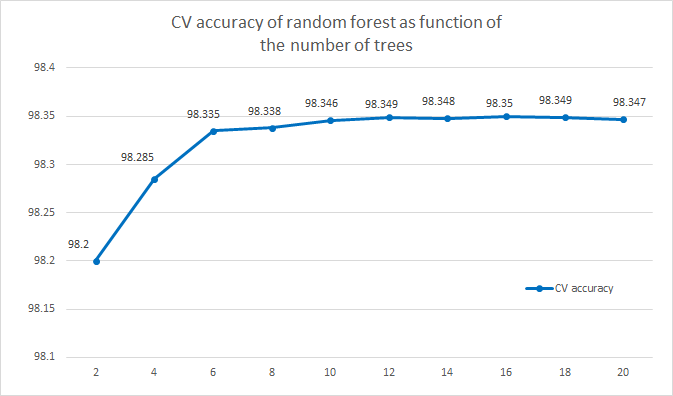
\includegraphics[width=8.5cm]{RFestimator.png}}
%  \vspace{2.0cm}
\end{minipage}
\label{fig:RFestimator}
\caption{CV accuracy of Random forest with varying number of estimators}
\end{figure}
\begin{figure}[htb]
\begin{minipage}[b]{1.0\linewidth}
  \centering
  \centerline{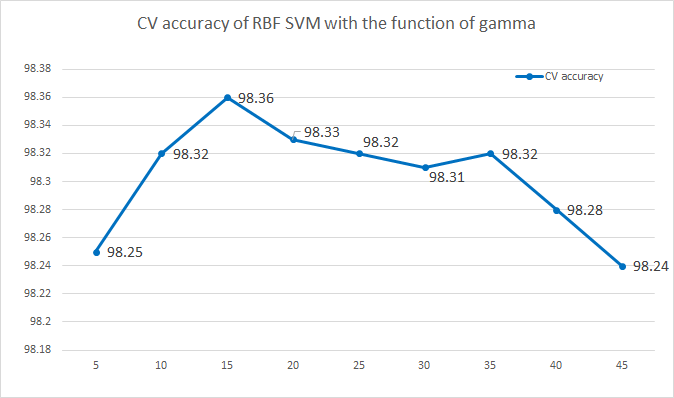
\includegraphics[width=8.5cm]{RBFSVMgamma.png}}
%  \vspace{2.0cm}
\end{minipage}
\label{fig:RBFSVMgamma}
\caption{CV accuracy of RBF SVM with varying $\gamma$.}
\end{figure}
\subsubsection{Comparison of classifiers}
Our last experiment involves quantitative comparison between 3 types of classifiers: RF, linear SVM and RBF SVM on two best found feature sets. The comparison is shown in Figure 3.4.3.
\begin{figure}[htb]
\begin{minipage}[b]{1.0\linewidth}
  \centering
  \centerline{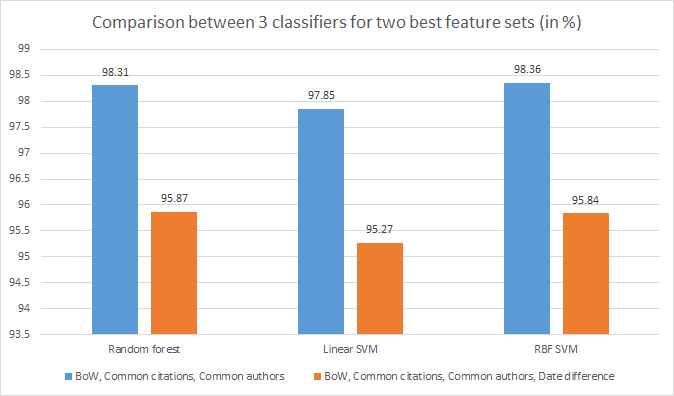
\includegraphics[width=8.5cm]{classifier.png}}
%  \vspace{2.0cm}
\end{minipage}
\label{fig:classifier}
\caption{CV accuracy of Random forest with varying number of estimators}
\end{figure}
For separate feature types in our first step. There is not any dominance between 3 classifiers for the best parameter sets. The random forest sometimes outperforms SVM classifier in some cases. However, for the combinations of features. The RBF SVM always has the best performance and the next one is linear SVM.
\section{Some methods that did not work out}
\label{sec:notwork}
In this section, we present some methods that we tried but did not work well.
\begin{itemize}
\item \textbf{Addressing the synonyms by Word2Vec:} A problem that needs to be addressed is how to cluster synonyms. In all abstracts, there are words that are synonyms of each others. They may have similar meaning (e.g. problematic, troublesome) or in sigular/plural forms (e.g. package, packages.) One major problem the we faced when trying to cluster is that the dataset does not contain a sufficiently large amount of text to feed into a Word2Vec mode. Therefore, we used an alternative solution: reuse a Word2Vec pre-trained model by Google in \cite{word2vecgg}. But this type of feature still did not have a significant contribution to the final model. The CV accuracy is lower than the individual common author feature.
\item \textbf{The use of Doc2Vec \cite{DBLP:LeM14}:} We also tried to capture some correlation between two document in each pair by a Doc2Vec model whose library is available in gensim 0.10.3. This approach also did not work out. A possible explanation is that at the level of text meaning, two papers that are cited in a pair do not share much correlation. Our use of Doc2Vec could not capture much difference between a cited and non-cited pair.
\item \textbf{Citation link prediction of old and theoretical papers:} As mentioned above, our prediction of a link is mainly based on the similarity in a text and in a network. In reality, there may be the case when we have a paper which is quite old and is in a completely different domain but contains a significant theory for the current paper that cites to. This is the case that we could not handle well because almost all features that we chose favor the papers that are closely related to each other.
\end{itemize}

\section{Conclusion}
\label{sec:conclusion}
In the scope of this project, we managed to build a model that predicts the links based on the choice of appropriate features and classifiers. The criterion to choose the feature is the contribution to the performance of the system. Final result shows that graph features play a significant role in link prediction and must be present in the final chosen features. Text features does not have a big contribution when being used alone but when being combined with graph features, it can improve the performance of the model comparing with the use of only graph features.\\
One of the drawback of our approach lies at the feature selection. Due to the need for determining the best classifier for each feature set, this process is almost infeasible to conduct completely automatically. We hope to find a better solution in the near future.

% References should be produced using the bibtex program from suitable
% BiBTeX files (here: strings, refs, manuals). The IEEEbib.bst bibliography
% style file from IEEE produces unsorted bibliography list.
% -------------------------------------------------------------------------
\bibliographystyle{IEEEbib}
\bibliography{biblio.bib}

\end{document}